% http://fachschaft.physik.uni-dortmund.de/images/GlobaltutAP/protokoll.txt
% ========================================
%	Header einbinden
% ========================================

% http://fachschaft.physik.uni-dortmund.de/images/GlobaltutAP/apheader.txt
% ==================================================
%	Festlegung der Dokumentenklasse
% ==================================================


\documentclass[paper=a4, 		% Layout für DinA4
	ngerman				% Deutsche Spracheinstellungen
	]
	{scrartcl} 			% Dokumentklasse für Aufsätze oder z.B. Praktikumsprotokolle

\usepackage{fixltx2e}			% Behebt ein paar Fehler in Latex

% ==================================================
%	Einstellen des Encodings
% ==================================================

\usepackage{ifxetex}
\usepackage{ifluatex} 

\ifxetex
	\usepackage{fontspec}
  	\usepackage{xunicode}
	\usepackage{xltxtra}
    \defaultfontfeatures{Mapping=tex-text} 	% To support LaTeX quoting style
	\setmainfont{Linux Libertine}
=======
    \defaultfontfeatures{Mapping=tex-text} % To support LaTeX quoting style
	\setmainfont{Linux Libertine} % Hier gewünschte Schriftart einfügen
\else
	\ifluatex
		\usepackage{fontspec}		% Falls das nicht funktioniert: \usepackage{luainputenc}
  		\usepackage{xunicode}
  		\defaultfontfeatures{Mapping=tex-text} % To support LaTeX quoting style
		\setmainfont{Linux Libertine} % Hier gewünschte Schriftart einfügen
	\else %pdfTeX
	  \usepackage[utf8]{inputenc}
	  \usepackage[T1]{fontenc}
	 \fi
\fi


% ==================================================
%	Spracheinstellungen
% ==================================================

\usepackage[ngerman]{babel,		% neue deutsche Rechtschreibung
	varioref}			% Bei Referenzen wird der Name des Objektes vor die Refernznummer geschrieben: z.B. \ref{bsp} liefert Seite 1

% ==================================================
%	Referenzen und Links
% ==================================================

\usepackage{hyperref}			% Verlinkungen innerhalb und außerhalb des PDF-Dokuments
\usepackage{url}			% Formattiert URLs, so dass sie sich z.B. besser vom Text abheben
\urlstyle{tt}				% TrueType-Schrift für URLs		



% ==================================================
%	Bibliograhphie
% ==================================================
%Zwei verschiedene Möglichkeiten Bibliographien einzubinden:

%	Möglichkeit 1:
% ========================
	\usepackage[numbers]{natbib}	%Paket für Bibliograhien

	%Bibtex: Nachnamen in Kapitälchen
	%\renewcommand*{\mkbibnamelast}[1]{\textsc{#1}}
	\newcommand*{\mkbibnamelast}[1]{\textsc{#1}}

	% Makros für Anhang + Referenzen
	\newcommand{\anhang}{
		\clearpage		% Anhang auf eine extra Seite packen
		\setcounter{page}{0}	
		\pagenumbering{Roman}	% Anhang wird in römischen Seitenzahlen numeriert
		\appendix		% Kapitelnummerierung in Großbuchstaben statt Zahlen.
	}

	\newcommand{\referenzen}{
		\bibliographystyle{alphadin} 			% Alphabetisch sortiert im DIN-Format
		\addcontentsline{toc}{section}{Referenzen}
		\phantomsection					% Referenzen ins Inhaltsverzeichnis
		\renewcommand{\refname}{\section*{Referenzen}\vspace*{-1em}} % Benennt das Kapitel um
		\bibliography{../include/Bibliographie.bib} 	% Die BibTeX-Datei einbinden
	}
%Zu Verwenden mit \bibliography{BIBDATEI}
% ========================
%	Möglichkeit 2:
% ========================
	%\usepackage{csquotes}				%Wird für Biblatex benötigt
	%\usepackage[style=alphabetic]{biblatex}	%Paket für Bibliograhphien mit Biblatex
%Zu Verwenden mit \bibliography{BIBDATEI} und \printbibliography oder \printbibliography[heading=bibintoc] (falls ein Inhaltsverzeichns verwendet wird)
% ==================================================



% ==================================================
%	Grafiken, Abbildungen und Tabellen
% ==================================================

\usepackage{graphicx}                   % zum Einbinden von Grafiken
\usepackage{xcolor}			% Für die Verwendung von Farben
\usepackage[font=small,			% kleine Schrift für Bildunterschriften
	labelfont=bf			% Fettgedruckte Bildunterschriften
	]
	{caption}			% Für Bildunterschriften

\usepackage{subcaption}			% Für mehrere Objekte nebeneinander mit eigenen Bildunterschriften

\usepackage{tabularx}			% Erweiterte Befehle für Tabellen
\usepackage{booktabs}			% Für professionele Tabellen, siehe Manual
\usepackage{longtable}			% Für Tabellen, die nicht mehr auf eine Seite passen.

\usepackage{rotating}			% Zum Verdrehen von Objekten. Nur mäßig verwenden.

%\graphicspath{{figs/}{bilder/}}	% Bildverzeichnisse MUSS ÜBERPRÜFT WERDEN!!!

% ==================================================
%	Mathematikumgebungen und Einheiten
% ==================================================

\usepackage{amsmath}			% Paket für mathematische Umgebungen und Funktionen
\usepackage{amsfonts}			% Zusätzliche Mathematische Schriftarten
\usepackage{amssymb}			% Zusätzliche Mathematische Symbole
%\usepackage{amscd}			% Zum Setzen Kommutativer Diagramme
\usepackage{amstext}			% Textsatz in der Matheumgebung
\usepackage{upgreek}			% Aufrechte griechische Buchstaben


% Diagramme mit tikz und Gnuplot zeichnen
%	\usepackage{tikz}
%	\usepackage{tikz-qtree}
%	\usepackage{gnuplot-lua-tikz}

% ==================================================
% SIUnitX: Einheiten werden vollautomatisch gesetzt
% ==================================================
\usepackage[
    separate-uncertainty = true, 		% Stellt den Fehler separat dar: Siehe SIUnitX-Manual
    mode 			= text, 	% Stellt Einheiten (Kelvin etc.) Nichtkursiv dar
    quotient-mode	= 	fraction,	% Bruchstriche nutzen
    repeatunits           = false, 
    range-phrase          = {\,bis\,},  
]{siunitx}
\sisetup{
	per-mode = fraction, 			% Bruchstriche nutzen
	output-decimal-marker = {,}, 		% Setzt das Dezimaltrennzeichen als Komma
	multi-part-units = brackets,
	exponent-product = \cdot,
}

\addto\extrasgerman{\sisetup{locale = DE}}	% "Deutsche" Einheiten
\usepackage{cancel}				% Kürzen von Einheiten in SIUnitX ermöglichen


% ==================================================
%	Sonstiges
% ==================================================

%\usepackage[official]{eurosym}			% offizielles Eurosymbol

% ==================================================
%	Seitenlayout
% ==================================================

% Kein Einrücken der Absätze (Einrücken = Null)
	\setlength{\parindent}{0pt}             % kein Einrücken der ersten Zeile in einem neuen Absatz

% Vermeidung von "Schusterjungen"
	\clubpenalty = 3000			% Höchstwert 10000, dann dürfen theoretisch keine Schusterjungen mehr auftreten.
% Vermeidkung von "Hurenkindern"
	\widowpenalty = 3000			% Höchstwert 10000, dann dürfen theoretisch keine Hurenkinder mehr auftreten.
	\displaywidowpenalty = 3000		% Es werden beide Einstellungen benötigt.

% Seitenlayout ändern mit Fancy
	\usepackage{fancyhdr}			% Paket zum bequemeren Verändern des Seitenlayouts

	% Tabellen ändern:
		\renewcommand{\thetable}{\arabic{section}.\arabic{table}} % figures bekommen die richtige Nummerierung: x.y
		\makeatletter \@addtoreset{table}{section} \makeatother      % nach jeder section wird neu gezählt

	% Kapitelüberschriften in der Kopfzeile:
		\renewcommand*{\sectionmark}[1]{\markboth{}{\thesection\ #1}}
		%\renewcommand*{\subsectionmark}[1]{\markboth{}{\thesubsection\ #1}}
		\renewcommand*{\subsectionmark}[1]{\markboth{}{}} % keine Unterüberschriften in der Kopfzeile
		\renewcommand{\plainheadrulewidth}{0.4pt}
	
	% Seitennummern rechts in der Kopfzeile:
		\lhead[\fancyplain{\thepage}{\thepage}]{\fancyplain{}{\rightmark}}
		\rhead[\fancyplain{}{\leftmark}]{\fancyplain{\thepage}{\thepage}}
	
	%Fußzeilen bleiben leer
		\lfoot{}
		\cfoot{}
		\rfoot{}
		
%Eigenes
\usepackage[section]{placeins} %use \FloatBarrier to keep pictures or tables in front of barrier
\renewcommand*\rmdefault{iwona}\normalfont\upshape

% ========================================
%	Angaben für das Titelblatt
% ========================================

\title{Versuch 402 - Dispersionsmessungen am Glasprisma\\				% Titel des Versuchs 
\large TU Dortmund, Fakultät Physik\\ 
\normalsize Anfänger-Praktikum}

\author{Oliver Zietek\\			% Name Praktikumspartner A
{\small \href{oliver.zietek@tu-dortmund.de}{oliver.zietek@tu-dortmund.de}}	% Erzeugt interaktiven einen Link
\and						% um einen weiteren Author hinzuzfügen
Fabian Lehmann\\					% Name Praktikumspartner B
{\small \href{fabian.lehmann@tu-dortmund.de}{fabian.lehmann@tu-dortmund.de}}		% Erzeugt interaktiven einen Link
}


\date{20. Dezember 2012}				% Das Datum der Versuchsdurchführung

% ========================================
%	Das Dokument beginnt
% ========================================

\begin{document}

% ========================================
%	Titelblatt erzeugen
% ========================================

\maketitle					% Jetzt wird die Titelseite erzeugt
\thispagestyle{empty} 				% Weder Kopfzeile noch Fußzeile

% ========================================
%	Der Vorspann
% ========================================

%\newpage					% Wenn Verzeichnisse auf einer neuen Seite beginnen sollen
%\pagestyle{empty}				% Weder Kopf- noch Fußzeile für Verzeichnisse

\tableofcontents

%\newpage					% eine neue Seite
%\thispagestyle{empty}				% Weder Kopf- noch Fußzeile für Verzeichnisse
%\listoffigures					% Abbildungsverzeichnis

%\newpage					% eine neue Seite
%\thispagestyle{empty}				% Weder Kopf- noch Fußzeile für Verzeichnisse
%\listoftables					% Tabellenverzeichnis
\newpage					% eine neue Seite


% ========================================
%	Kapitel
% ========================================

%\section{Einleitung}				% Bei Bedarf
%	%
%

\section{Theorie}
	%picdispkurve,picapparatur,picsymstrahl,picprismawinkel,picbrechwinkel
%eqbrech, eqdispcurve, eqdisp1, eqdisp2
\subsection{Brechung und Dispersion}
	\begin{figure}[h]
		\begin{center}
		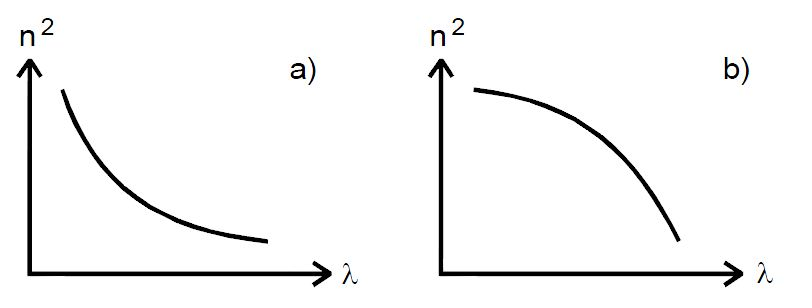
\includegraphics[scale=0.7]{picdispkurve.jpg}
		\caption{Gestalt möglicher Dispersionskurven[1]}
		\label{picdispkurve}
		\end{center}	
	\end{figure}
Durch Wechselwirkungen mit Elektronen ist die Geschwindigkeit von Licht in Materie
geringer als die Vakuumslichtgeschwindigkeit. Dadurch kommt es zu Brechungen an 
Materiegrenzflächen nach Gleichung (\ref{eqbrech}) mit dem Brechungsindex $n$.
Da die Ausbreitungsgeschwindigkeit von der Wellenlänge $\lambda$ des Lichtes abhängt, 
wird Licht unterschiedlicher Frequenz verschieden stark gebrochen. Dieses
Phänomen wird Dispersion genannt. Eine Abhängigkeit nach (\ref{eqdispkurve})
heißt Dispersionskurve\cite{anleitung} (vgl. Abb. \ref{picdispkurve}).
\begin{align}
n&=\frac{v_1}{v_2} \label{eqbrech} \\
v_1&, v_2 : \text{materialabhängige Geschwindigkeit von Licht} \nonumber \\
n&=f(\lambda) \label{eqdispkurve}
\end{align}
Aus dem Huygensschen Prinzip lässt sich das Snelliussche Brechungsgesetz (Gl. (\ref{eqsnellius})) folgern,
bei einem Eintritt unter einem Winkel $\alpha$ folgt mit dem Brechungsindex $n$ ein
Austrittswinkel $\beta$.
\begin{align}
n&=\frac{sin \alpha}{sin \beta}\label{eqsnellius}
\end{align}
\subsection{Dispersion an einem Prisma}
Unter Annahme eines Strahlendurchgangs von sichtbarem Licht von Luft in
ein durchsichtiges, farbloses Material lassen sich Dispersionsgleichungen \cite{anleitung} ableiten:
Gilt für die Absorbtionsstelle $\lambda_1$ mit der Wellenlänge $\lambda$ im Vakuum, dass $\lambda>>\lambda_1$,
so gilt Gleichung (\ref{eqdisp1}), welche in Abbildung \ref{picdispkurve} als a) dargestellt ist.
Gilt hingegen $\lambda<<\lambda_1$, so gilt Gleichung (\ref{eqdisp2}), welche in Abbildung \ref{picdispkurve} 
als b) dargestellt ist. Beide Kurven beschreiben normale Dispersion, also Abnahme von $n$ bei Zunahme von $\lambda$.
\begin{align}
n^2(\lambda)&=A_0+\frac{A_2}{\lambda^2}+\frac{A_4}{\lambda^4}+\ldots \text{ mit } A_i>0 \label{eqdisp1} \\
n^2(\lambda)&=1-A_2' \lambda^2-A_4'\lambda4-\ldots \text{ mit } A_i'>0, i\geq 2 \label{eqdisp2}
\end{align}
\subsection{Prismenspektralapparat}
	\begin{figure}[h]
		\begin{center}
		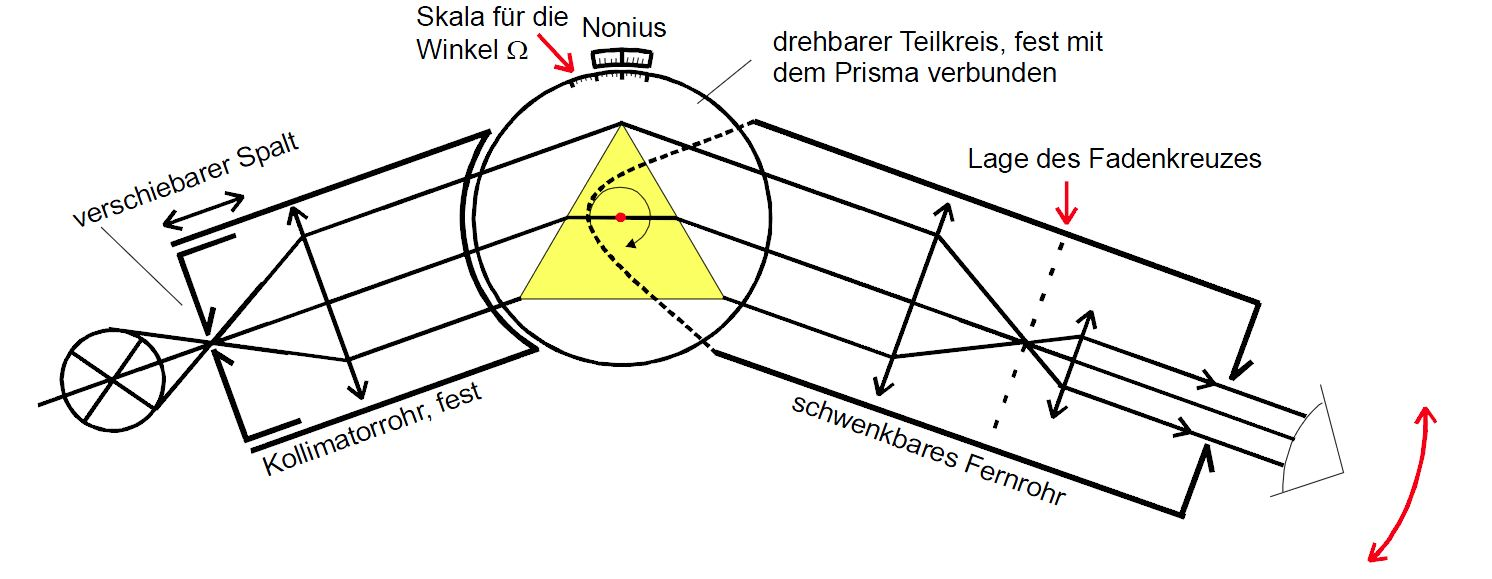
\includegraphics[scale=0.3]{picapparatur.jpg}
		\caption{Schematische Darstellung des Prismenspektralapparates[1]}
		\label{picapparatur}
		\end{center}	
	\end{figure} 	\begin{figure}[h]
		\begin{center}
		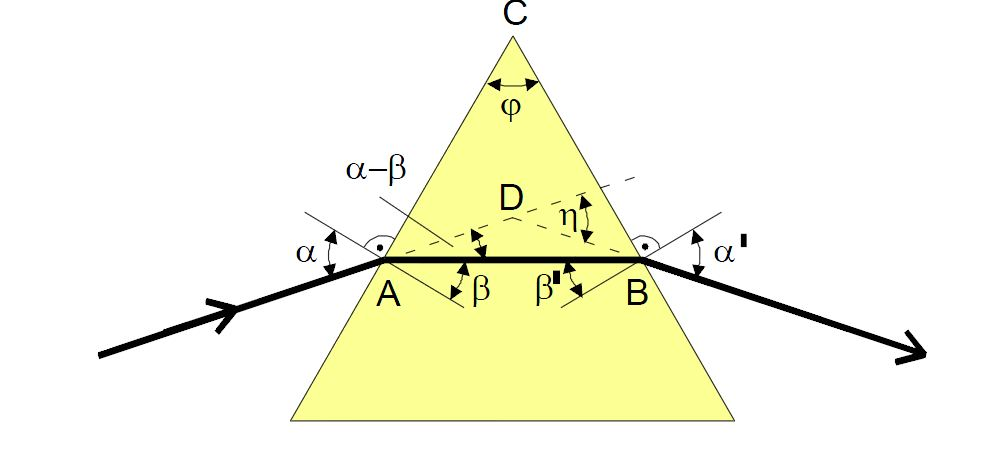
\includegraphics[scale=0.4]{picsymstrahl.jpg}
		\caption{Symmetrischer Strahlengang durch ein Prisma[1]}
		\label{picsymstrahl}
		\end{center}	
	\end{figure}
Mit Hilfe eines Prismenspektralapparates (siehe Abb. \ref{picapparatur}) lässt sich der Brechungsindex 
abhängig von der Wellenlänge durch ABlesen von Winkeln bestimmen. Das Gerät macht sich das Snelliussche Brechungsgesetz zu nutze,
bei dem symmetrischen Durchgang des Lichtstrahls (Abb. \ref{picsymstrahl}) lässt sich folgende Gleichung 
herleiten.
\begin{align}
n&=\frac{sin\frac{\eta + \phi}{2}}{\frac{\phi}{2}}\\
\text{ mit }\alpha&=\frac{\eta + \phi}{2}
\end{align}
\subsection{Bestimmung des Brechungswinkels zwischen brechenden Oberflächen des Prismas}
	\begin{figure}[h]
		\begin{center}
		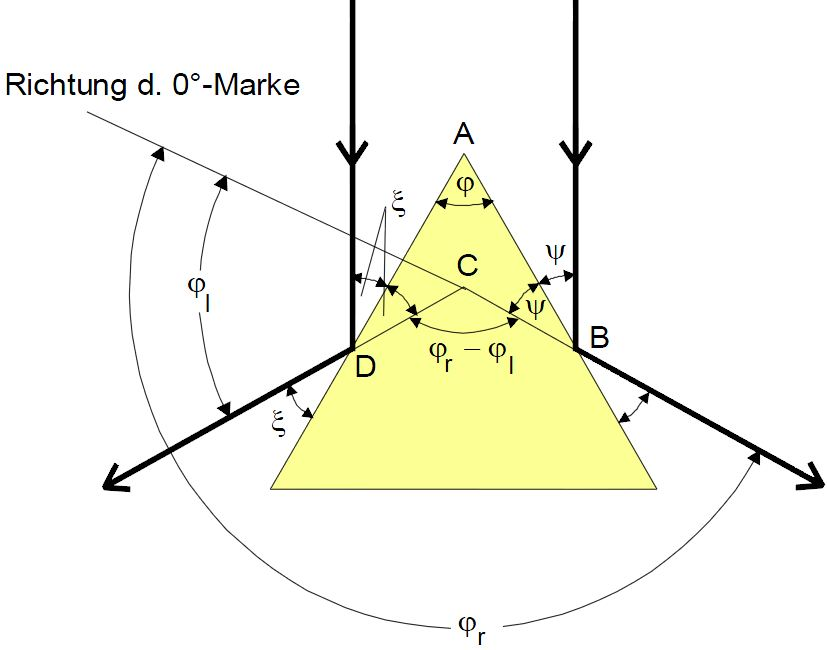
\includegraphics[scale=0.3]{picprismawinkel.jpg}
		\caption{Bestimmung des Winkels zwischen den brechenden Oberflächen[1]}
		\label{picprismawinkel}
		\end{center}	
	\end{figure}
Wird das Prisma wie in Abbildung \ref{picprismawinkel} ausgerichtet, kann aus einfachen
Winkelbeziehungen durch Messen der Reflektionswinkel beider Lichtstrahlen der brechende 
Winkel $\phi$ des Prismas bestimmt werden.
\begin{align}
\phi&=\frac{1}{2}(\phi_r - \phi_l)
\end{align}
\subsection{Bestimmung der Brechungswinkel der Spektrallinien}
	\begin{figure}[h]
		\begin{center}
		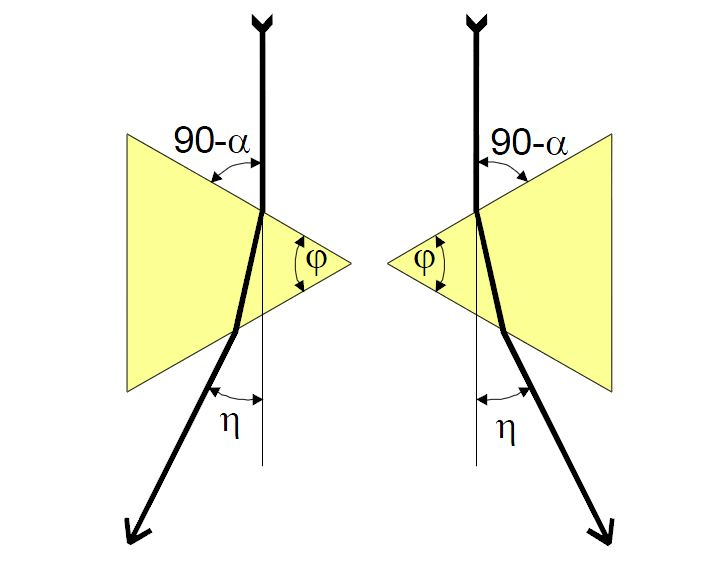
\includegraphics[scale=0.3]{picbrechwinkel.jpg}
		\caption{Brechwinkelbestimmung mit spiegelbildlicher Prismenstellung[1]}
		\label{picbrechwinkel}
		\end{center}	
	\end{figure}
Aus zwei zueinander spiegelsymmetrischen Stellungen des Prismas können die Brechungswinkel
bestimmt werden. Bei dem Zusammenfallen der gebrochenen Lichtstrahlen mit dem reflektierten
Lichtstrahl lässt sich mit Abbildung \ref{picbrechwinkel} folgende Beziehung ableiten.
\begin{align}
\eta&=180-(\Omega_r-\Omega_l)
\end{align}
	\FloatBarrier
\section{Durchführung}
	%
%
\subsection{Bestimmung des Brechungswinkels zwischen brechenden Oberflächen des Prismas}
Das Prisma wird mit der brechnenden Kante ungefähr auf das Kollimatorrohr ausgerichtet (vgl. Abb. \ref{picprismawinkel}).
Dann werden die Reflektionswinkel mit dem Fernrohr gemessen. Dieser Vorgang wird mehrfach für die verschiedenen Kanten wiederholt.
\subsection{Bestimmung der Brechungswinkel der Spektrallinien}
Das Prisma wird so lange gedreht, bis die jeweilige Farbe des gebrochenen Lichtspektrums mit dem reflektierten Lichtstrahl
zusammenfällt. Dann wird das Prisma in eine spiegelsymmetrische Stellung gebracht und der Vorgang wird wiederholt (vgl. Abb. \ref{picbrechwinkel}).
	\FloatBarrier
\section{Auswertung}
	\subsection{Bestimmung der Brechungsindices}

Zur Messung des Brechnungsindex benutzen wir einen Prismenspektralapparat.
Dabei ist ein Glasprisma auf dem Drehteil eines Goniometers montiert. Durch
einen Spalt und eine Sammellinse fällt Licht aus einer Heliumlampe auf
das Prisma. Dadurch, dass der Spalt in der Brennebene der Linse steht, erhalten
wir paralleles Licht. Nach der Brechung fällt das Licht in die Brennebene einer Lupe, durch welche wir
die Spektrallinien sehen können.
Da wir nur den symmetrischen Fall betrachten, bei dem a = a' und b = b'
ist, folgt
\begin{align}
n=\frac{sin(\frac{\varphi + \eta}{2})}{sin(\frac{\varphi}{2})}\nonumber
\end{align}

Um sicherzustellen, dass ein symmertrischer Strahlenverlauf vorliegt, bringt
man den gebrochenen Strahl mit dem an der Basis des Prismas reflektrierten
Strahl zur Deckung. Dann misst man die Auslenkung des gebrochenen Strahles
links und rechts und berechnet den Brechnungswinkel wie folgt:

\begin{align}
-\eta=180^\circ +\Omega_l - \Omega_r \nonumber
\end{align}

Weiterhin sollte der Winkel an der brechenden Kante gemessen. Dafür wurde
diese Kante auf das Kollimatorrohr gerichtet und der Winkel des reflektierten
Strahles gemessen. Dieser Winkel wurde auf beiden Seiten fünf mal abgelesen,
wobei das Prisma mit der brechenden Kante über den Strahl hinweg auf eine
spiegelverkehrte Position gedreht wurde. Damit ergibt sich mit der Formel:

\begin{align}
\varphi=180^\circ +\varphi_l - \varphi_r \nonumber
\end{align}

\begin{table}[h]
\begin{center}
\begin{tabular}[c]{|c|c|c|} \hline
$\varphi_l$ in $^\circ$ & $\varphi_r$ in $^\circ$ & $\varphi$  in $^\circ$\\ \hline
263,9 & 23,6+360 & 60,3 \\ 
229,2 & 349,2 & 60 \\ 
229,5 & 349,3 & 60,2 \\ 
241,4 & 1,5+360 & 60,1 \\ 
240,0 & 360,0 & 60,3 \\ \hline
\end{tabular}
\caption{Winkel $\Phi$ an der brechenden Kante des Prismas}
\end{center}
\end{table}
% \newpage

Somit lautet der Mittelwert:
$\varphi = 60, 18^\circ \pm 0, 58^\circ$ Der Fehler wird mit der Formel der Standardabweichung des Mittelwertes
berechnet.

Für die Indicies n und $\eta$ folgt damit:
\begin{table}[h]
\begin{center}
\begin{tabular}[c]{|c|c|c|c|c|c|} \hline
Farbe & $\lambda$ in nm & $\Omega_l$  in $^\circ$ & $\Omega_r$  in $^\circ$ & $\eta$  in $^\circ$ & n \\ \hline
Rot & 632,8 & 147,5 & 27,5 +360 & 60 & 1,729\\
Gelb & 594,1 & 147,3 & 27,2+360 & 59,9 & 1,728\\
Gr"un & 543,5 & 146,8 & 26,7+360 & 59,9 & 1,728\\
Blau & kA & 146,4 & 26,2+360 &  59,8 & 1,727\\ \hline
\end{tabular}
\caption{Brechungsindicies n und $\eta$}
\end{center}
\end{table}

\subsection{Bestimmung der Dispersionskurve}

Um die Dispersionskurve zu bestimmen, werden die Quadrate der Brechungsindize
gegen Quadrate der Wellenlängen und einmal gegen die Kehrwerte der Wellenlängenquadrate.
Somit kann man mit einer linearen Regression y = mx + b bestimmen, durch die Abweichung der
Kurve von den Messwerten kann bestimmt werden, welche Dispersionskurve die richtige ist.
Aus der Ausgleichsrechnung ergibt sich für $n^2$ gegen $\lambda^{-2}$ 
 \begin{align}
n^2( \lambda ) = (-0,302 \pm 0,241) \mu m^{2} \lambda^{-2} + 2,996 \pm 0,007\nonumber
\end{align}
und für $n^2$ gegen $\lambda^2$ ergibt sich
\begin{align}
n'^2( \lambda ) = (0,273 \pm 0,183) \mu m^{-2} \lambda^2 + 2,977 \pm 0,006 \nonumber
\end{align}

Durch die berechnung der Abstandsquadrate $s_n$ und $s_n'$ folgt die richtige Dispersionskurve.
 \begin{align}
s_n=2,3043\nonumber
\end{align}
\begin{align}
s_n'=0,0193\nonumber
\end{align}
Woraus folgt, dass die Dispersionskurve die gültige ist und folgendermaßen aussieht:

\begin{figure}[h]
	\centering
		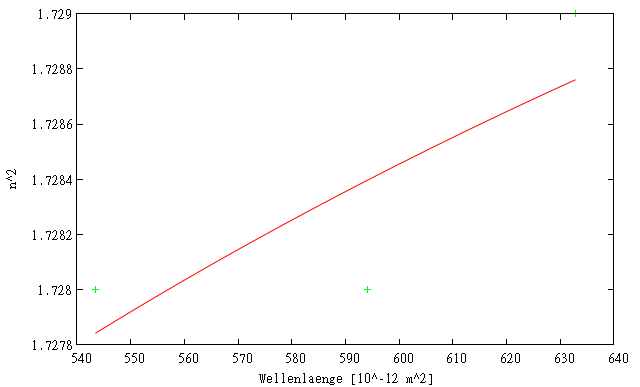
\includegraphics[width=1.00\textwidth]{Plot1B.png}
		\caption{Dispersionskurve}
	\label{fig:Plot}
\end{figure}

\subsection{Bestimmung der Abbesche Zahl}
Zur Berechung der Abbeschen Zahl benötigt man die Formel
\begin{align}
v=\frac{n_D-1}{n_F-n_C}\nonumber
\end{align}
Für die man die Brechungsindizes der FRAUNHOFER'schen Linien benötigt. Diese erhält man
indem man $\lambda_C$= 656nm,$\lambda_D$ = 589nm und $\lambda_F$ = 486nm in die Formel einsetzt.
Dabei muss man beachten, dass $A_0$ und $A_2$ fehlerbehaftet sind, da die Messergebnisse,wie in der Diskussion
erläutert große Fehler aufweisen wird auf die Fehlerfortpflanzung an dieser Stelle verzichtet.

Somit folgt:

\begin{align}
n_C= 2,294\nonumber
\end{align}
\begin{align}
n_D= 2,125\nonumber
\end{align}
\begin{align}
n_F= 1,717\nonumber
\end{align}
\begin{align}
v= -1,950 \nonumber
\end{align}





	\FloatBarrier
\section{Diskussion}
	%
%
\subsection{Statistische Fehler}
Die Messung lies einige statistische Fehler zu:

1. Die Apparatur verwackelt bei Drehung des Fernrohres und des Prisma.

2.Die Spektrallinien können nicht als idealisiert betrachtet werden, da man einen Spalt
endlicher Breite hat.

3. Der Raum war nicht richtig abgedunkelt bzw. die im Raum befindlichen Lichtquellen,
wie Leselampen, haben den Versuch beeinflusst.

4. Auf der Apparatur befindet sich teilweise Staub. Sowohl auf dem Prisma, als auch auf
den optischen Bauteilen des Fern- und Kollimatorrohres.

Die Messung des Winkels $\varphi$ zwischen den Oberflächen war mit $59,96^\circ \pm 0,04^\circ$ im Bereiches der erwarteten $60^\circ$ des Prismas, Abweichungen lassen sich auf statistische Fehler beim Messvorgang zurückführen.
Zusätzlich gab es nur wenige Punkte die ausgewertet werden konnten, da die Lichtverhältnisse mehr nicht zuließen. Auch dies führte zu weiteren Ungenauigkeiten.
\subsection{Grundsätzliche Ungenauigkeiten}
Neben diesen apparaturbedingten Fehlern ist ein grundsätzlicher Fehler unterlaufen, als ein gespiegeltes 
Spektrum ausgemessen wurde. Dies ließ sich jedoch aufgrund einfacher geometrischer Zusammenhänge wieder auf das eigentlich
zu messende Spektrum schließen. \\
Die Abbesche Zahl,
\begin{align}
v&=50\pm10,
\end{align}
sowie das theoretische Auflösungsvermögen für $\lambda_C$ und $\lambda_F$,
\begin{align}
A_C&=1530\pm80,\text{ }A_F=3400\pm500,
\end{align}
sind verhältnismäßig ungenau. Den ebenso wie die Berechnung der Absroptionsstelle,
\begin{align}
\lambda_i&=(114\pm 6)\text{ nm},
\end{align}
 beruhen die Werte auf den Anfangs errechneten Werten der auch nur genäherten Dispersionskurve. 
 Wenn diese Anfangswerte nun aber aus ungenau gemessenen, teilweise erst noch gespiegelten Messwerten 
 errechnet worden sind, so sind darauf folgende Werte mit einem mindestens gleich großen Fehler behaftet. 
	\FloatBarrier
% ========================================
%	Literaturverzeichnis
% ========================================
\nocite{link1} \nocite{link2}
\bibliographystyle{plainnat}			% Bibliographie-Style auswählen
\bibliography{lit}			% Literaturverzeichnis

% ========================================
%	Das Dokument endent
% ========================================
%\includegraphics[scale=0.75]{img011.jpg}
\end{document}